
\section{Lo sviluppo di una memoria locale}

La visualizzazione di un elemento comporta il recupero dei suoi dati, 
necessari per mostrare le informazioni desiderate.
Attualmente questa funzionalità è realizzata effettuando una chiamata al server
ogni volta che viene richiesto un dato.
Chiedere, ottenere ed elaborare dati dal server richiede però tempo e risorse,
causando ritardi che impattano sulle prestazioni e sull'esperienza utente.
Inoltre, questo rende l'utilizzo l'applicazione strettamente dipendente dalla sua connessione al server,
che diventa così inutilizzabile in situazioni in cui il dispositivo non abbia modo di comunicare.\\
\\
È quindi utile salvare copie degli elementi usati più frequentemente 
nella memoria locale del dispositivo,
nel caso in cui tecnologia del dispositivo lo permetta.
In questa maniera, nel momento in cui un'interazione richieda la visualizzazione dei dati, 
si possono fornire immediatamente le informazioni disponibili in copia, 
senza la necessità di utilizzare un'ulteriore richiesta.
Questo permette la diminuzione del carico del server, 
una maggiore reattività del prodotto e una migliore esperienza utente.\\
\\
La creazione e la persistenza delle copie deve essere gestita 
in maniera trasparente rispetto alla logica grafica, 
creando nell'applicazione utente un livello intermedio tra 
la visualizzazione delle informazioni e la comunicazione con il server.
Questo livello sarà incaricato di gestire la persistenza e la modalità di recupero dei dati,
fornendoli quando richiesti, 
nascondendo la complessità derivata dalla necessità di allineare le due memorie.\\
\\
Inoltre, data la natura condivisa dell'applicazione risulta fondamentale 
che l'aggiornamento avvenga quanto più possibile in tempo reale rispetto modifiche applicate:
oltre a essere una prerogativa di tutte le applicazioni moderne, 
ne viene influenzata anche la user experience. 
Lo spostamento di un appuntamento, 
la conferma di una presenza o la modifica del luogo di appuntamento 
sono elementi critici per i quali gli utenti devono venire informati il prima possibile. \\
\\
Tutto questo comporta sfide progettuali che permettano di garantire allo stesso tempo 
sia la correttezza dei dati presenti che il loro allineamento all'interno del minor ritardo possibile.
\clearpage
\subsection{La realizzazione della cache}
Per motivi di prestazioni,
Flutter mantiene nativamente lo stato di un componente 
solo per il tempo strettamente necessario per la sua fruizione. 
Normalmente il tempo di vita del suo stato coincide quindi 
con quello del componente a cui è associato. 
Se si correlasse questa logica con il mantenimento dei dati,
la persistenza locale degli elementi e dei dati avrebbe durata limitata,
comportando la richiesta delle informazioni al server 
ogni volta che si vuole visualizzare un elemento. 
Si rende perciò necessaria la creazione e la gestione di una memoria locale 
indipendente dalle logiche grafiche,
che permetta di mantenere i dati ricevuti dal server 
anche in seguito al termine del servizio dei componenti.\\
\\
Gli elementi mantenuti in cache devono essere unici e disponibili in tutto il programma.
I dati verranno salvati in collezioni di oggetti corrispondenti alle classi logiche del dominio, 
la cui gestione universale sarà affidata a servizi dedicati. 
L'esecuzione dei servizi dovrà essere indipendente dall'interfaccia,
fornendo l'accesso agli elementi delle collezioni,
ma gestendo anche le loro modifiche.
In caso alcuni elementi subiscano dei cambiamenti (dal dispositivo stesso o tramite notifica), 
sarà inoltre compito loro aggiornare i componenti coinvolti.
Per venire incontro a queste necessità, 
Flutter mette a disposizione dei componenti di tipologia provider,
ai quali i vari componenti grafici possono essere associati.\\
\begin{figure}[h!]
    \centering
    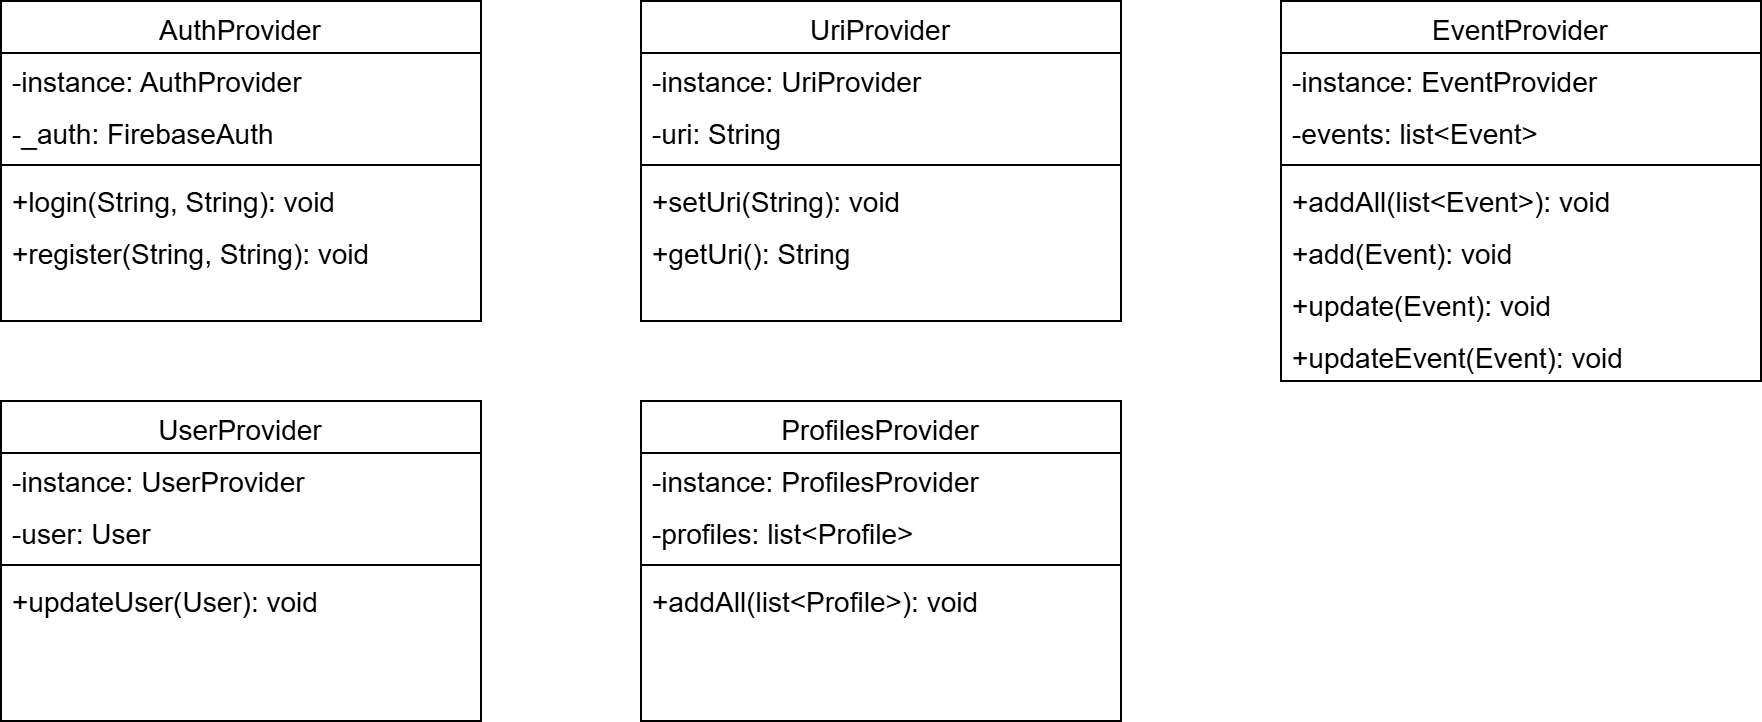
\includegraphics[height=.27\textheight]{FrontProviderClassDiagram.png}
    \caption{Classi provider all'interno dell'applicazione}
\end{figure}	
\\
Grazie all'associazione che si viene così a creare tra componenti grafici e provider,
questi ultimi hanno la possibilità di ricaricare attivamente parti del progetto, 
aggiornandole nel momento in cui avviene una modifica che li coinvolge.
Questo genera una pulizia generale del codice,
integrando e nascondendo tutta la logica di collegamento e distribuzione degli eventi.
Per ogni entità principale del dominio è stata associata una collezione,
che viene gestita da un provider apposito.
Nel momento in cui un componente deve visualizzare un elemento,
dichiara la sua dipendenza con il servizio provider relativo, 
a cui farà richiesta per i dati.
Nel caso in cui i dati siano già presenti in memoria verranno restituiti subito.
Altrimenti la grafica li sostituirà temporaneamente con elementi neutri,
in attesa della risposta.
All'arrivo della risposta il provider notifica l'elemento grafico, 
che si aggiorna di conseguenza.
L'unicità delle collezioni e dei rapporti con il server è ottenuta 
grazie all'implementazioni dei provider come classi singleton,
pattern di sviluppo che garantisce la cardinalità di una classe 
in al massimo un'istanza per ogni momento.\\
\begin{figure}[h!]
    \centering
    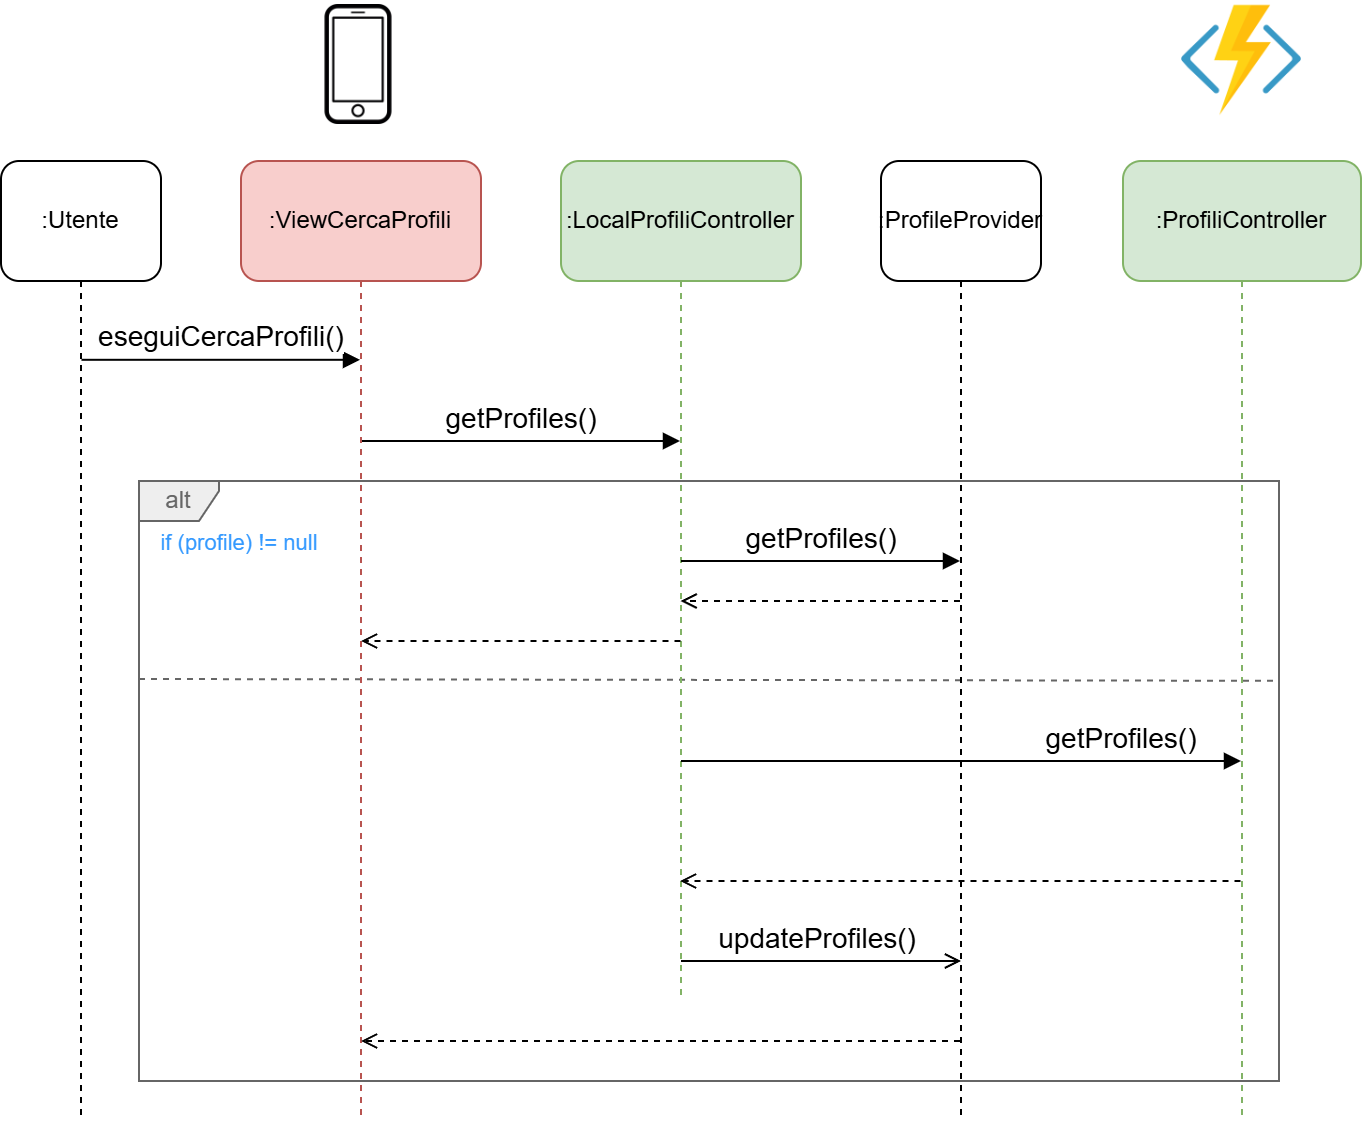
\includegraphics[height=.5\textheight]{PICercaProfili.png}
    \caption{Esempio di interazione logica tra i componenti del client}
\end{figure}
\clearpage
I vantaggi dell'implementazione di una memoria locale
derivano dalla sua capacità di rimanere aggiornata con il server principale.
Risulta infatti inutile facilitare l'accesso a dei dati 
se questi, una volta forniti, risultano scorretti.
Per essere sicuri che la cache possa quindi essere considerata valida in ogni momento
è necessario implementare strategie che, 
all'interno di un intervallo di tolleranza,
garantiscano l'allineamento con i dati presenti sul server.
La principale fonte di aggiornamenti viene fornita direttamente dal server che,
attraverso un processo di comunicazioni in tempo reale,
invia delle notifiche ai client ogni qual volta vengano interessati da una modifica.\\

\subsection{La scelta della tecnologia per la comunicazione in tempo reale}
La comunicazione con il server finora implementata 
si basa sul protocollo Hypertext Transfer Protocol (HTTP). 
HTTP prevede un fornitore di servizi (il server) mettere a disposizione una porta 
a un indirizzo fisso rimanendo in attesa di eventuali utilizzatori (client) che, 
interfacciandosi attivamente alla porta disponibile, espongono le loro richieste.
La riduzione delle comunicazioni al minimo indispensabile, 
oltre a non richiedere al server alcuna conoscenza del client, 
rende il protocollo pratico e scalabile.\\
\\
Questa dinamica però impedisce ai client di essere notificati di eventuali modifiche apportate, 
a meno di richieste periodiche frequenti che comportano un sovraccarico da entrambe le parti. 
Inoltre, l’inversione dei ruoli non è applicabile 
in quanto i client cambiano costantemente l’indirizzo a loro associato, 
così come è impossibile distinguere se il dispositivo abbia terminato la connessione
o se abbia subito un guasto di altro tipo. \\
\\
Si necessita una comunicazione che mantenga in costante contatto 
i client con le modifiche del server, 
permettendo una trasmissione attiva degli aggiornamenti.
A basso livello, il protocollo più adatto per permettere una comunicazione continua 
tra le tecnologie comunemente diffuse è quello delle WebSocket. 
Tramite WebSocket infatti si crea un canale diretto tra le parti 
che consente una comunicazione istantanea.\\
\\
Alla necessità di supportare il protocollo delle WebSocket e di inviare istantaneamente i messaggi,
si aggiunge la possibilità di creare molteplici canali specifici 
per indirizzare correttamente le comunicazioni ai soli interessati.\\
\\
Per individuare la tecnologia più adatta ad aggiornare gli utenti, 
tra le tante che offrono servizi di collegamento istantaneo tra tecnologie, 
è fondamentale comprendere  gli scopi per cui sono nate e che problemi quindi risolvono. 
Infatti, ogni servizio è stato progettato per affrontare specifiche sfide che si differenziano 
sia per la natura dei servizi a cui si rivolgono che per le loro modalità di utilizzo.\\
\begin{figure}[h!]
    \centering
    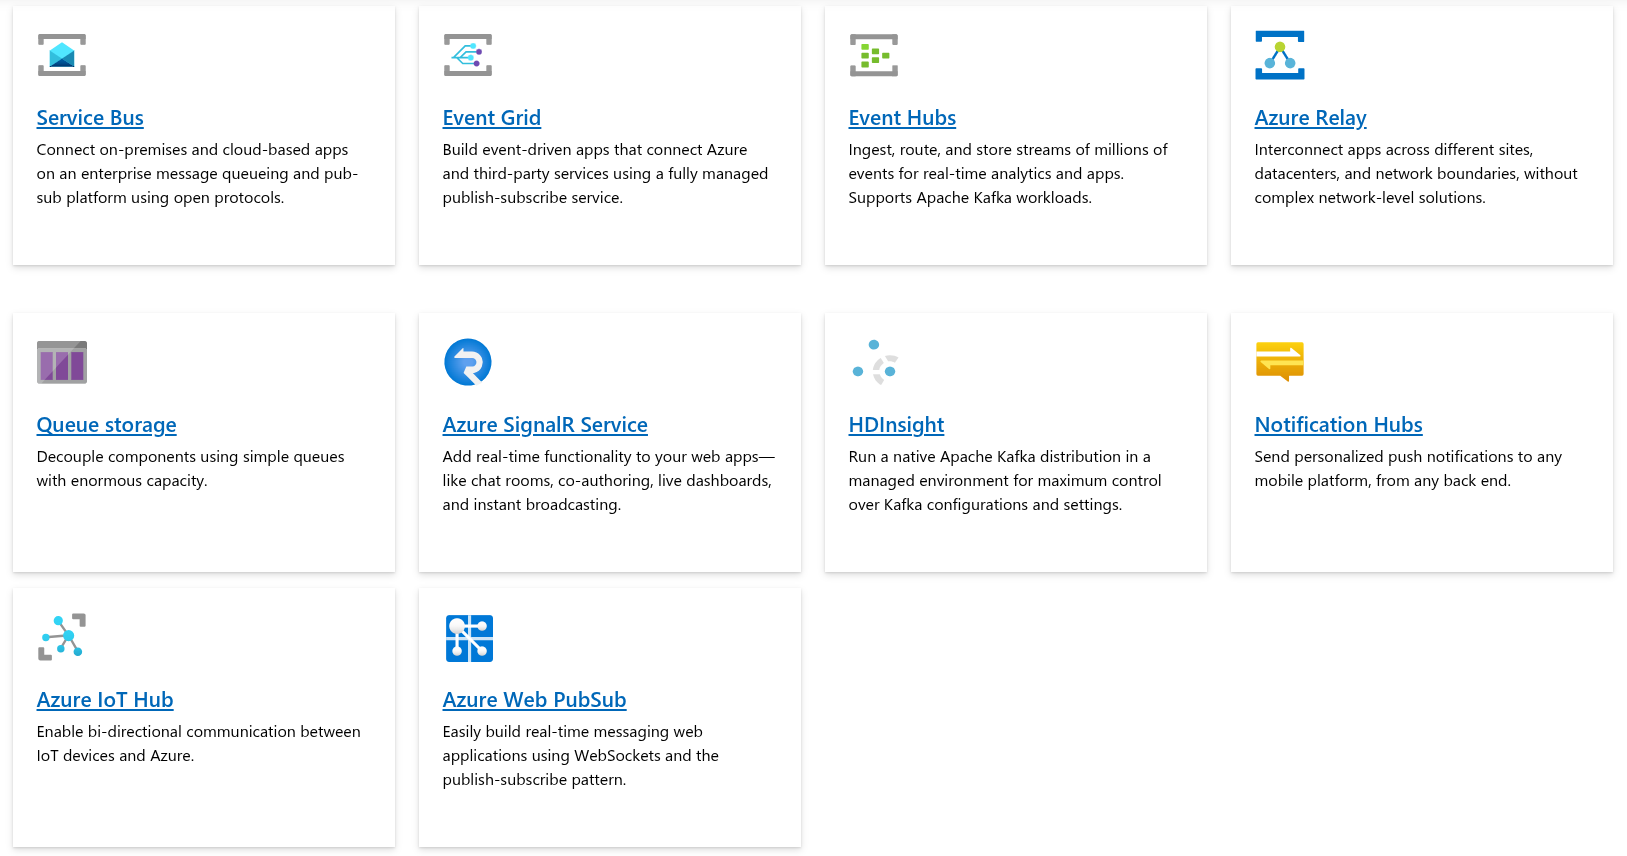
\includegraphics[width=\textwidth]{AzureMessagingServices.png}
    \caption{I servizi di comunicazione istantanea proprietari di Azure}
\end{figure}	\\
La natura degli attori per cui il servizio si specializza 
determina le prestazioni di scalabilità e le integrazioni supportate. 
Bisogna quindi considerare la località e la natura delle risorse: in-premise o sul cloud, 
se appartengono alla stessa piattaforma o se devono comunicare internamente.
Ad esempio, un servizio pensato per collegare tantissimi dispositivi distribuiti con limitato potere computazionale, 
come nel caso dell’Internet of Things, fornirà  supporto a connessioni esterne e a protocolli standard, 
e prevederà un’elevata quantità di richieste di limitate dimensioni e frequenza. 
Viceversa, la necessità di creare una comunicazione tra un numero ristretto di server con prestazioni elevate 
comporta la creazione di flussi di dati importanti, 
magari gestiti internamente all’ambiente cloud, astraendo la tecnologia necessaria.\\
\\
I servizi si differenziano però anche per le caratteristiche delle connessioni gestite.
Proprietà fondamentale è la natura delle comunicazioni. 
I canali possono essere infatti unidirezionali, 
permettere la comunicazione da entrambe le parti o implementati come flussi di eventi, 
in cui le comunicazioni possono essere inviate e ricevute da molteplici attori, 
senza che il destinatario sia noto al mittente. 
Inoltre, alcuni servizi offrono la possibilità di individuare categorie di clienti specifiche 
a cui eventualmente inviare notifiche mirate. 
Infine, bisogna prendere in considerazione la necessità di persistenza delle comunicazioni, 
che fornisce, oltre all’aggiornamento in tempo reale, 
anche la possibilità di recuperare modifiche passate.\\
\\
Nel progetto si necessita di un servizio che supporti le WebSocket 
e che permetta di creare una molteplicità di canali unidirezionali differenti. 
In particolare, deve essere il più indipendente possibile dagli attori 
con cui comunica per poter garantire il maggior supporto possibile. 
Dovendo coprire solo le notifiche di aggiornamento, 
senza responsabilità di rintracciabilità dei dati, 
la presenza della persistenza non è necessaria.\\
\begin{wrapfigure}{r}{0.25\textwidth}
    \centering
    
\includegraphics[height=.12\textheight]{pubsub.png}
    Azure PubSub
\end{wrapfigure}
Gratuito per le prime 20 connessioni, 
ma eventualmente scalabile per soddisfare ulteriori carichi, 
il servizio individuato per la gestione delle notifiche in tempo reale è Azure Web Pub Sub (AWPS). 
Permette infatti la creazione di canali tramite WebSockets e l'integrazione con le Azure Functions. 
Supporta la creazione di canali, sia unidirezionali che bidirezionali, su cui pubblicare eventi, 
a cui gli utenti possono collegarsi per ricevere gli aggiornamenti. 
Non prevede il supporto alla persistenza, 
inviando direttamente i messaggi senza mantenerli in memoria,
ma gestisce la scalabilità del sistema.\\

\subsection{L'invio delle notifiche}

L'integrazione di Azure Web Pub Sub deve avvenire
sia a livello server che con i device degli utenti. 
Seguendo il modello publish subscribe, ogni client creerà una connessione con AWPS in sola lettura, 
ricevendo tutti i dati che lo interessano. 
Il server avrà il compito di interfacciarsi con il servizio 
per pubblicare i dati sui canali.
Un canale è un contenitore logico che rappresenta 
un argomento a cui un utente può essere interessato.
Un dispositivo può essere associato a più canali, 
pur mantenendo la stessa connessione.\\
\\
Le modifiche verranno inviate ai canali,
che le propagheranno a loro volta a tutti i dispositivi collegati. 
La scelta della definizione dell'elemento in base al quale il canale viene creato 
deriva da un'ulteriore analisi del dominio. 
Il soggetto interessato alle modifiche sottoposte a notifica è il profilo.
Dunque verranno creati i canali relativamente ai profili.
Un dispositivo descrive però l'interazione di un utente.
Per questo motivo, una volta creata la connessione con il servizio,
il dispositivo si iscrive ai canali dei profili associati al suo utente.\\
\\
\mycomment{sicurezza}
Se però si creassero i canali in relazione ai profili ogni dispositivo 
(che riassume l'interazione di un utente) dovrebbe mantenere una connessione per ogni profilo collegato all'utente. 
La creazione di un canale per ogni device allo stesso modo risulta estremamente inefficiente, 
in quanto, oltre a introdurre nuovi requisiti per garantire la tracciabilità dei dispositivi, 
ne richiederebbe di creazione e gestione in numero elevato. 
Per queste ragioni i canali verranno creati uno per utente, 
garantendo inoltre che gli unici utenti a ricevere 
le notifiche ne posseggano effettivamente l'accesso adeguato.\\
\\
A seguito di una richiesta che comporta una modifica
che necessita di essere propagata ai profili interessati,
il server avrà il compito di interfacciarsi con AWPS per affidargli le comunicazioni relative. 
Tuttavia AWPS non supporta la capacità di unire gli elementi in base alle loro relazioni, 
se non quelle tra gli utenti e i profili definite implicitamente dai canali. 
Per questo motivo, è molto probabile che l'operazione di notifica richieda una richiesta al database, 
per recuperare i profili coinvolti.
Ad esempio, la modifica di un evento comporta la notifica a tutti i profili relativi, 
e quindi sarà necessario recuperare tutti i profili associati a quell'evento.\\
\\
Vista la responsabilità precisa e considerato che 
l'effettivo invio delle notifiche non è un'operazione essenziale 
per il successo di una richiesta,
si delega questo compito a un'altra funzione.
Questa funzione avrà quindi il compito di recuperare i profili coinvolti
per mettersi poi in contatto con AWPS e per pubblicare le notifiche sui relativi canali.
A differenza delle funzioni chiamate per garantire la consistenza della persistenza principale,
dove era essenziale garantire il controllo e il successo dell'operazione, 
in questo caso si preferisce ottenere uno svolgimento veloce senza 
che questo richieda tutto il carico aggiuntivo derivato dal controllo del risultato,
considerando accettabile la sua eventuale perdita o fallimento.\\
\begin{wrapfigure}{r}{0.25\textwidth}
    \centering
    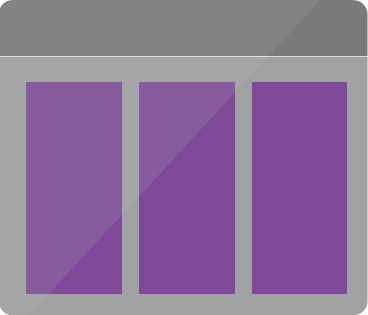
\includegraphics[height=.12\textheight]{queue.png}
    Azure Storage Queue
\end{wrapfigure}
Queste considerazioni hanno portato alla scelta di Azure Storage Queue
come strumento di delega per le operazioni di notifica.
Offre infatti un servizio veloce ed economico, 
sebbene non fornisca nativamente un meccanismo di controllo 
che garantisca il successo dell'operazione legata al messaggio.
Al termine della sua esecuzione la funzione principale aggiungerà quindi
a una coda dedicata un messaggio con le informazioni relative 
alla modifica da lei apportata.
Una seconda funzione, la cui attivazione è collegata all'aggiunta di oggetti in quella coda,
leggerà il messaggio, per poi eseguire il recupero dei profili e il collegamento con AWPS.\\
\begin{figure}[htpb]
    \centering
    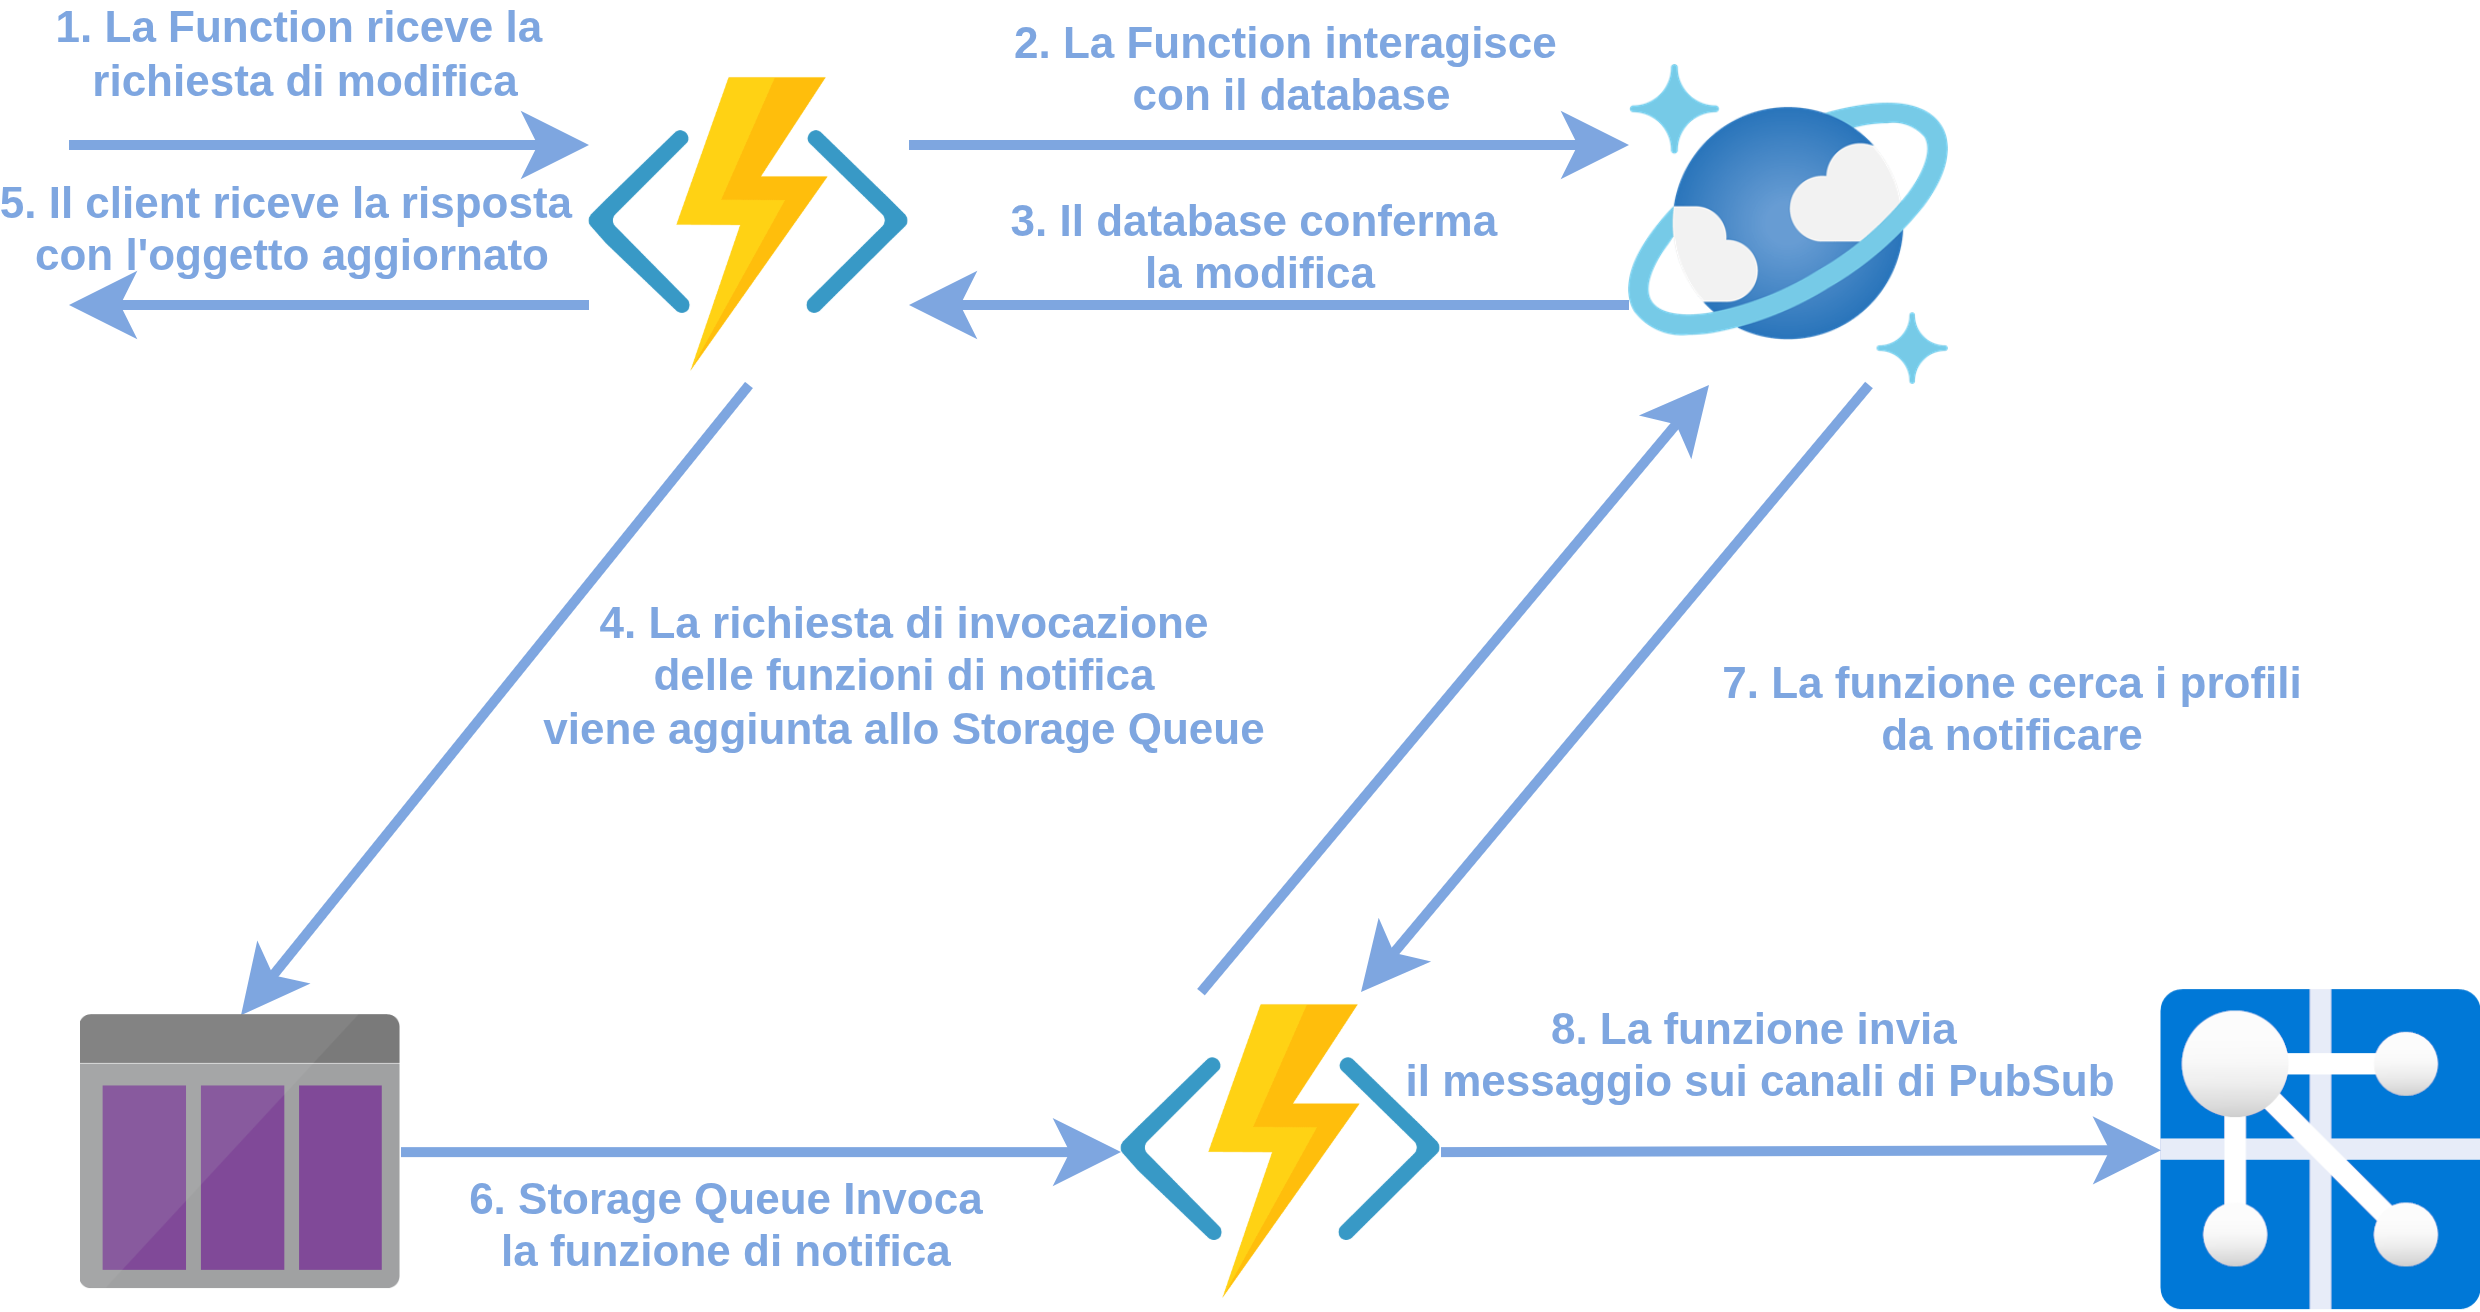
\includegraphics[width=\textwidth]{NotificationsSchema.png}
    \caption{Interazione delle Azure Functions con la Queue}
\end{figure}
\clearpage
Nell'ottica di rendere il processo di invio delle notifiche 
il più veloce ed efficiente possibile, 
si è deciso di includere nel messaggio le informazioni minime sull'accaduto.
Questo permette di uniformare il formato delle notifiche, 
semplificando la loro gestione e velocizzando l'invio,
diminuendo il volume dei dati trasmessi tramite WebSocket.
Alla ricezione della notifica il client apporterà, se possibile,
gli aggiustamenti dovuti.
In caso di modifiche importanti sarà però sua responsabilità 
recuperare i dati aggiornati direttamente dalla memoria centrale.
Questa strategia risulta particolarmente efficace 
soprattutto in caso di 
numerose modifiche ravvicinate sullo stesso elemento, 
che possono essere raggruppate per poi eseguire la richiesta di aggiornamento una sola volta.\\
\begin{figure}[htpb]
    \centering
    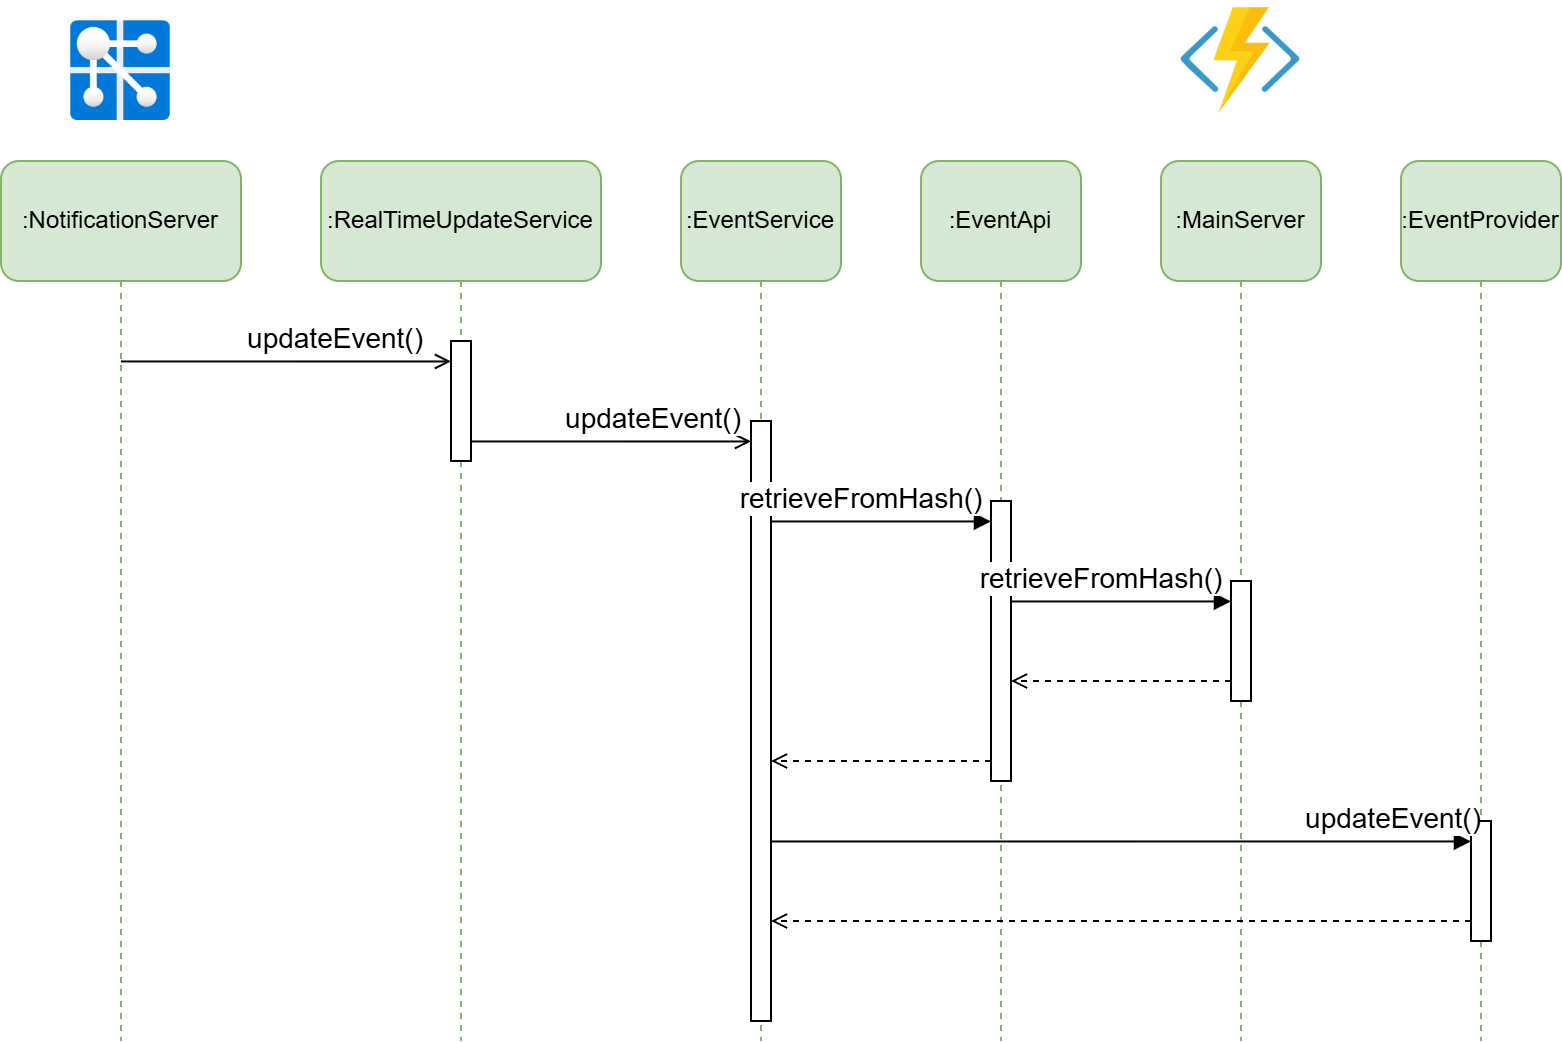
\includegraphics[width=\textwidth]{IIAggiornaEvento.png}
    \caption{Interazione tra AWPS e un client per il recupero di un Event}
\end{figure}	
\\
Per poter assicurare però che nessuna notifica sia andata persa
si necessita l'implementazione di un processo che
si confronti con il server per recuperare le modifiche non ricevute.\\
\clearpage
\subsection{Il processo per garantire l'allineamento della cache}

Il client ha la responsabilità di tenere allineata
la propria cache ai valori della memoria centrale. 
La presenza di dati aggiornati in cache permette infatti,
oltre a garantire tempi di reazione minimi,
di evitare di ricorrere a richiedere dati al server per ogni interazione utente, 
La validità selle risorse che ha salvato in cache,
nonostante la ricezione di notifiche, 
dipende dalla certezza che corrispondano integralmente ai dati ufficiali.\\
\\
La ricezione degli aggiornamenti tramite WebSocket e 
la loro dipendenza dalle Azure Storage Queue non garantiscono la loro consegna.
Come discusso nella precedente sezione infatti, 
non sono previsti ulteriori tentativi di esecuzione nel caso in cui 
la funzione incaricata dell'invio fallisca.
Inoltre, la tecnologia WebSocket, pur essendo veloce ed efficiente, 
può subire interruzioni o perdite dimostrandosi non completamente affidabile.
Per poter quindi considerare allineata la cache alla memoria centrale, 
si necessita di un processo che assicuri l'aggiornamento dei dati in memoria.\\
\\
A ogni elemento viene associato il momento relativo al suo ultimo aggiornamento noto.
Si tiene inoltre memoria dell'ultimo momento in cui è stata 
attivamente effettuata una richiesta esplicita di aggiornamento.  
A ogni avvio dell'applicazione il client invierà una richiesta al server 
per ricevere tutti gli elementi che hanno subito modifiche 
successivamente al momento dell'ultimo aggiornamento.
Alla ricezione della risposta si aggiorna il momento dell'ultima richiesta.\\
\\
Da quel momento in poi, periodicamente, 
verrà inviata una richiesta contenente sia gli identificativi che il momento dell'ultimo aggiornamento 
degli elementi le cui modifiche sono giunte al dispositivo (grazie alle notifiche) durante l'ultimo intervallo.
Il server, ricevendo queste informazioni, controllerà se combaciano con tutte le entità 
associate al profilo della richiesta.
In caso trovi incongruenze, ovvero emergano elementi non presenti tra quelli ricevuti o 
con data di modifica successiva a quella dichiarata, 
restituirà suddetti elementi con gli ultimi dati aggiornati.\\
\\
\clearpage